% board.tex — Standard Chinese 飞行棋 (Aeroplane Chess) board
% Reconstructed from the user's exact 10-cell spec + 4 segment-head color rules
% + 5-rect/edge constraint.
%
% Geometry (user coordinate system: x right, y down):
%   - Board: 8.5 × 8.5 (NOT 9 — the +0.5 was excess width)
%   - C4 rotational center: (4.25, 4.25)
%   - 4 bases (2×2): NW red (0..2, 0..2), NE yellow (6.5..8.5, 0..2),
%                    SE blue (6.5..8.5, 6.5..8.5), SW green (0..2, 6.5..8.5)
%   - 4 cross arms (each 5 narrow rectangles in mid-arm):
%       top arm rectangles: 5 cells along (3..5.5, 0..1), each 0.5 × 1
%   - Outer loop: 56 cells (4 segments × 14 each = 1 takeoff + 13 track cells)
%   - Colors: 4-color cycle (green, red, yellow, blue) connected around the loop.
%       Segment head colors: red=green, yellow=red, blue=yellow, green=blue.
%   - 4 dashed long-flight lines, each connecting two same-color airplane
%     triangles (in opposite concave corners).
%
% Compile: pdflatex board.tex

\documentclass[border=12pt]{standalone}
\usepackage{tikz}
\usetikzlibrary{arrows.meta, calc}

\definecolor{redC}{HTML}{E33030}
\definecolor{yellowC}{HTML}{F5C518}
\definecolor{blueC}{HTML}{2074D6}
\definecolor{greenC}{HTML}{38A342}
\definecolor{parchment}{HTML}{FFFFFF}
\definecolor{ink}{HTML}{1F1F1F}

% Small white-circle marker on each non-takeoff track cell.
% Usage: \dot{x}{y}
\newcommand{\dotC}[2]{%
    \fill[white] (#1, #2) circle (0.18);%
    \draw[ink, line width=0.25pt] (#1, #2) circle (0.18);%
}

% Small plane glyph (triangle pointing in +x direction in local frame).
\newcommand{\planeG}[3]{%
    % #1 = cx, #2 = cy, #3 = color
    \begin{scope}[shift={(#1, #2)}]
        \fill[#3] (-0.16, 0.13) -- (0.21, 0) -- (-0.16, -0.13) -- cycle;
        \draw[ink, line width=0.25pt] (-0.16, 0.13) -- (0.21, 0) -- (-0.16, -0.13) -- cycle;
    \end{scope}
}

% Plane glyph with rotation: \planeR{cx}{cy}{rot}{color}
% rot=0   -> face right, =90 -> face up, =180 -> face left, =270 -> face down
% (Used for takeoff cells.)
\newcommand{\planeR}[4]{%
    \begin{scope}[shift={(#1, #2)}, rotate=#3]
        \fill[#4] (-0.16, 0.13) -- (0.21, 0) -- (-0.16, -0.13) -- cycle;
        \draw[ink, line width=0.25pt] (-0.16, 0.13) -- (0.21, 0) -- (-0.16, -0.13) -- cycle;
    \end{scope}
}

% Smaller triangle plane glyph (used on dashed-line direction indicators).
\newcommand{\planeRSmall}[4]{%
    \begin{scope}[shift={(#1, #2)}, rotate=#3]
        \fill[#4] (-0.10, 0.08) -- (0.13, 0) -- (-0.10, -0.08) -- cycle;
        \draw[ink, line width=0.2pt] (-0.10, 0.08) -- (0.13, 0) -- (-0.10, -0.08) -- cycle;
    \end{scope}
}

% Realistic airliner silhouette (option G):
% - Smooth Bezier-curve fuselage
% - Swept-back main wings
% - Smaller swept horizontal stabilizers at tail
% Used for stationary planes: concave-corner planes + planes parked in bases.
% Fits in 0.18-radius circle.
\newcommand{\planeIconBody}[1]{%
    \fill[#1]
        (0.17, 0)
        .. controls (0.16, 0.014) and (0.13, 0.026) .. (0.05, 0.028)
        -- (-0.12, 0.024)
        .. controls (-0.16, 0.020) and (-0.18, 0.010) .. (-0.18, 0)
        .. controls (-0.18, -0.010) and (-0.16, -0.020) .. (-0.12, -0.024)
        -- (0.05, -0.028)
        .. controls (0.13, -0.026) and (0.16, -0.014) .. (0.17, 0)
        -- cycle;
    \fill[#1] (0.04, 0.024) -- (-0.06, 0.14) -- (-0.12, 0.14) -- (-0.04, 0.024) -- cycle;
    \fill[#1] (0.04, -0.024) -- (-0.06, -0.14) -- (-0.12, -0.14) -- (-0.04, -0.024) -- cycle;
    \fill[#1] (-0.12, 0.020) -- (-0.14, 0.06) -- (-0.17, 0.055) -- (-0.15, 0.020) -- cycle;
    \fill[#1] (-0.12, -0.020) -- (-0.14, -0.06) -- (-0.17, -0.055) -- (-0.15, -0.020) -- cycle;%
}
\newcommand{\planeIcon}[3]{%
    \begin{scope}[shift={(#1, #2)}]
        \planeIconBody{#3}
    \end{scope}
}
\newcommand{\planeIconR}[4]{%
    \begin{scope}[shift={(#1, #2)}, rotate=#3]
        \planeIconBody{#4}
    \end{scope}
}
% Larger variant for in-base parked planes
\newcommand{\planeIconBig}[3]{%
    \begin{scope}[shift={(#1, #2)}, scale=1.6]
        \planeIconBody{#3}
    \end{scope}
}
\newcommand{\planeIconBigR}[4]{%
    \begin{scope}[shift={(#1, #2)}, rotate=#3, scale=1.6]
        \planeIconBody{#4}
    \end{scope}
}
% Smaller variant for concave-corner planes (flight-path endpoints)
\newcommand{\planeIconSm}[3]{%
    \begin{scope}[shift={(#1, #2)}, scale=0.8]
        \planeIconBody{#3}
    \end{scope}
}
\newcommand{\planeIconSmR}[4]{%
    \begin{scope}[shift={(#1, #2)}, rotate=#3, scale=0.8]
        \planeIconBody{#4}
    \end{scope}
}

\begin{document}
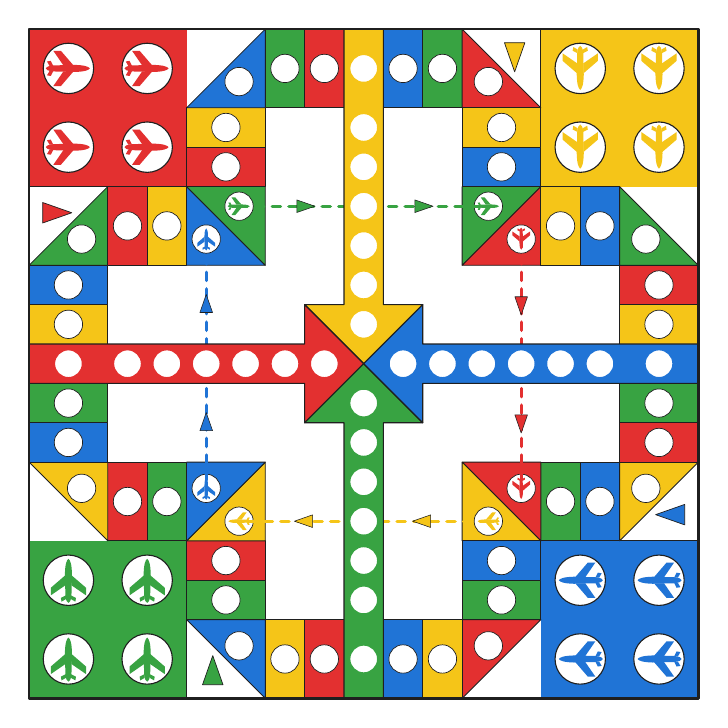
\begin{tikzpicture}[
    x={(1cm, 0cm)}, y={(0cm, -1cm)},
    every node/.style={font=\sffamily\footnotesize},
    line cap=round, line join=round,
]

    % ============================================================
    % 1. Background
    % ============================================================
    \fill[parchment] (0, 0) rectangle (8.5, 8.5);

    % ============================================================
    % 2. Four corner bases (2×2 each)
    % ============================================================
    \fill[redC]    (0,   0)   rectangle (2,   2);
    \fill[yellowC] (6.5, 0)   rectangle (8.5, 2);
    \fill[blueC]   (6.5, 6.5) rectangle (8.5, 8.5);
    \fill[greenC]  (0,   6.5) rectangle (2,   8.5);

    % ============================================================
    % 3. Parking circles + plane glyphs in each base
    %    (2×2 layout, plane direction = CW play direction after takeoff)
    % ============================================================
    % Red NW — face RIGHT
    \foreach \cx/\cy in {0.5/0.5, 1.5/0.5, 0.5/1.5, 1.5/1.5} {
        \fill[white] (\cx, \cy) circle (0.32);
        \draw[ink, line width=0.4pt] (\cx, \cy) circle (0.32);
        \planeIconBig{\cx}{\cy}{redC}
    }
    % Yellow NE — face DOWN (rotate=270) per user spec
    \foreach \cx/\cy in {7/0.5, 8/0.5, 7/1.5, 8/1.5} {
        \fill[white] (\cx, \cy) circle (0.32);
        \draw[ink, line width=0.4pt] (\cx, \cy) circle (0.32);
        \planeIconBigR{\cx}{\cy}{270}{yellowC}
    }
    % Blue SE — face LEFT (rotate=180)
    \foreach \cx/\cy in {7/7, 8/7, 7/8, 8/8} {
        \fill[white] (\cx, \cy) circle (0.32);
        \draw[ink, line width=0.4pt] (\cx, \cy) circle (0.32);
        \planeIconBigR{\cx}{\cy}{180}{blueC}
    }
    % Green SW — face UP (rotate=90)
    \foreach \cx/\cy in {0.5/7, 1.5/7, 0.5/8, 1.5/8} {
        \fill[white] (\cx, \cy) circle (0.32);
        \draw[ink, line width=0.4pt] (\cx, \cy) circle (0.32);
        \planeIconBigR{\cx}{\cy}{90}{greenC}
    }

    % ============================================================
    % 4. Outer loop — 4 segments × 14 cells each, drawn via C4 rotation.
    %    \cA..\cM = colors for k=1..13 of the segment.
    %    Red segment offset 0:    green, red, yellow, blue, green, red, yellow, blue, green, red, yellow, blue, green
    %    Yellow segment offset 1: red, yellow, blue, green, red, yellow, blue, green, red, yellow, blue, green, red
    %    Blue segment offset 2:   yellow, blue, green, red, yellow, blue, green, red, yellow, blue, green, red, yellow
    %    Green segment offset 3:  blue, green, red, yellow, blue, green, red, yellow, blue, green, red, yellow, blue
    % ============================================================
    % Note: TikZ rotate around inside x={(1,0)},y={(0,-1)} renders visually CCW
    % (top -> left for rotate=+90), so:
    %   rotate=0    -> NW (red segment)
    %   rotate=+90  -> SW (green segment, head color blue)
    %   rotate=+180 -> SE (blue segment, head color yellow)
    %   rotate=+270 -> NE (yellow segment, head color red)
    \foreach \rot/\cA/\cB/\cC/\cD/\cE/\cF/\cG/\cH/\cI/\cJ/\cK/\cL/\cM in {%
        0/greenC/redC/yellowC/blueC/greenC/redC/yellowC/blueC/greenC/redC/yellowC/blueC/greenC,
        90/blueC/greenC/redC/yellowC/blueC/greenC/redC/yellowC/blueC/greenC/redC/yellowC/blueC,
        180/yellowC/blueC/greenC/redC/yellowC/blueC/greenC/redC/yellowC/blueC/greenC/redC/yellowC,
        270/redC/yellowC/blueC/greenC/redC/yellowC/blueC/greenC/redC/yellowC/blueC/greenC/redC%
    } {
        \begin{scope}[rotate around={\rot:(4.25, 4.25)}]
            % idx 0: takeoff (white, no border at the hypotenuse to feel "open")
            \fill[white] (0, 2) -- (1, 2) -- (0, 3) -- cycle;
            \draw[ink, line width=0.3pt] (0, 2) -- (1, 2);
            \draw[ink, line width=0.3pt] (0, 2) -- (0, 3);

            % idx 1 (k=1): triangle (0..1, 2..3) right-bottom half
            \fill[\cA] (1, 2) -- (1, 3) -- (0, 3) -- cycle;
            \draw[ink, line width=0.3pt] (1, 2) -- (1, 3) -- (0, 3) -- cycle;
            \dotC{0.667}{2.667}

            % idx 2 (k=2): rectangle (1..1.5, 2..3)
            \fill[\cB] (1, 2) rectangle (1.5, 3);
            \draw[ink, line width=0.3pt] (1, 2) rectangle (1.5, 3);
            \dotC{1.25}{2.5}

            % idx 3 (k=3): rectangle (1.5..2, 2..3)
            \fill[\cC] (1.5, 2) rectangle (2, 3);
            \draw[ink, line width=0.3pt] (1.5, 2) rectangle (2, 3);
            \dotC{1.75}{2.5}

            % idx 4 (k=4): concave triangle (2..3, 2..3) left-bottom — flight glyph anchor
            % Position shifted from centroid (2.333, 2.667) to (2.25, 2.667) so that
            % the flight dashed line passes through the perpendicular stretch's 4th circle.
            % Radius unified to 0.18 (matching other track circles).
            \fill[\cD] (2, 2) -- (2, 3) -- (3, 3) -- cycle;
            \draw[ink, line width=0.3pt] (2, 2) -- (2, 3) -- (3, 3) -- cycle;
            \fill[white] (2.25, 2.667) circle (0.18);
            \draw[ink, line width=0.25pt] (2.25, 2.667) circle (0.18);

            % idx 5 (k=5): concave triangle (2..3, 2..3) right-top — flight glyph anchor
            % Position shifted from (2.667, 2.333) to (2.667, 2.25), radius 0.18.
            \fill[\cE] (2, 2) -- (3, 2) -- (3, 3) -- cycle;
            \draw[ink, line width=0.3pt] (2, 2) -- (3, 2) -- (3, 3) -- cycle;
            \fill[white] (2.667, 2.25) circle (0.18);
            \draw[ink, line width=0.25pt] (2.667, 2.25) circle (0.18);

            % idx 6 (k=6): rectangle (2..3, 1.5..2)
            \fill[\cF] (2, 1.5) rectangle (3, 2);
            \draw[ink, line width=0.3pt] (2, 1.5) rectangle (3, 2);
            \dotC{2.5}{1.75}

            % idx 7 (k=7): rectangle (2..3, 1..1.5)
            \fill[\cG] (2, 1) rectangle (3, 1.5);
            \draw[ink, line width=0.3pt] (2, 1) rectangle (3, 1.5);
            \dotC{2.5}{1.25}

            % idx 8 (k=8): convex triangle (2..3, 0..1) right-bottom
            \fill[\cH] (2, 1) -- (3, 1) -- (3, 0) -- cycle;
            \draw[ink, line width=0.3pt] (2, 1) -- (3, 1) -- (3, 0) -- cycle;
            \dotC{2.667}{0.667}

            % idx 9..13 (k=9..13): five 0.5×1 rectangles in mid-arm (3..5.5, 0..1)
            \fill[\cI] (3, 0) rectangle (3.5, 1);
            \draw[ink, line width=0.3pt] (3, 0) rectangle (3.5, 1);
            \dotC{3.25}{0.5}

            \fill[\cJ] (3.5, 0) rectangle (4, 1);
            \draw[ink, line width=0.3pt] (3.5, 0) rectangle (4, 1);
            \dotC{3.75}{0.5}

            \fill[\cK] (4, 0) rectangle (4.5, 1);
            \draw[ink, line width=0.3pt] (4, 0) rectangle (4.5, 1);
            \dotC{4.25}{0.5}

            \fill[\cL] (4.5, 0) rectangle (5, 1);
            \draw[ink, line width=0.3pt] (4.5, 0) rectangle (5, 1);
            \dotC{4.75}{0.5}

            \fill[\cM] (5, 0) rectangle (5.5, 1);
            \draw[ink, line width=0.3pt] (5, 0) rectangle (5.5, 1);
            \dotC{5.25}{0.5}
        \end{scope}
    }

    % ============================================================
    % 5. Plane glyphs on the 8 concave-corner triangles.
    %    Per segment: k=4 plane color = \cD, k=5 plane color = \cE.
    %    Direction: pointing toward the OTHER endpoint of the matching
    %    same-color dashed flight line.
    %
    %    Concave corners' centroids (rotated by C4):
    %    NW (red seg): k=4 (blue) at (2.333, 2.667), k=5 (green) at (2.667, 2.333)
    %    NE (yel seg): k=4 (green) at (5.917, 2.333), k=5 (red) at (6.167, 2.667)
    %      = rotate +90° around (4.25,4.25): (x,y)→(8.5-y, x)
    %      (2.333, 2.667) → (5.833, 2.333), (2.667, 2.333) → (6.167, 2.667)
    %    SE (blue seg): k=4 (red) at (6.167, 5.833), k=5 (yellow) at (5.833, 6.167)
    %    SW (green seg): k=4 (yellow) at (2.667, 6.167), k=5 (blue) at (2.333, 5.833)
    % ============================================================
    % Plane orientation rule (in this y-down picture):
    %   rotate=0   -> face right
    %   rotate=90  -> face up
    %   rotate=180 -> face left
    %   rotate=270 -> face down
    % User spec for concave-corner planes:
    %   NW (red base):    blue=up,    green=right
    %   NE (yellow base): green=right, red=down
    %   SE (blue base):   red=down,   yellow=left
    %   SW (green base):  yellow=left, blue=up
    %
    % NW — plane icons (preserving original arrow orientations)
    \planeIconSmR{2.25}{2.667}{90}{blueC}
    \planeIconSm{2.667}{2.25}{greenC}
    % NE
    \planeIconSm{5.833}{2.25}{greenC}
    \planeIconSmR{6.25}{2.667}{270}{redC}
    % SE
    \planeIconSmR{6.25}{5.833}{270}{redC}
    \planeIconSmR{5.833}{6.25}{180}{yellowC}
    % SW
    \planeIconSmR{2.667}{6.25}{180}{yellowC}
    \planeIconSmR{2.25}{5.833}{90}{blueC}

    % ============================================================
    % 6. Takeoff-cell plane glyphs (in the white triangle, same color as
    %    the base, pointing in CW play direction).
    %    Red takeoff centroid (0..1, 2..3 left-top half): (1/3, 7/3) ≈ (0.333, 2.333)
    % ============================================================
    % Red takeoff: face RIGHT (no rotation)
    \planeG{0.333}{2.333}{redC}
    % Yellow takeoff: face DOWN (rotate=270)
    \begin{scope}[shift={(6.167, 0.333)}, rotate=270]
        \fill[yellowC] (-0.16, 0.13) -- (0.21, 0) -- (-0.16, -0.13) -- cycle;
        \draw[ink, line width=0.25pt] (-0.16, 0.13) -- (0.21, 0) -- (-0.16, -0.13) -- cycle;
    \end{scope}
    % Blue takeoff: face LEFT (rotate=180)
    \begin{scope}[shift={(8.167, 6.167)}, rotate=180]
        \fill[blueC] (-0.16, 0.13) -- (0.21, 0) -- (-0.16, -0.13) -- cycle;
        \draw[ink, line width=0.25pt] (-0.16, 0.13) -- (0.21, 0) -- (-0.16, -0.13) -- cycle;
    \end{scope}
    % Green takeoff: face UP (rotate=90)
    \begin{scope}[shift={(2.333, 8.167)}, rotate=90]
        \fill[greenC] (-0.16, 0.13) -- (0.21, 0) -- (-0.16, -0.13) -- cycle;
        \draw[ink, line width=0.25pt] (-0.16, 0.13) -- (0.21, 0) -- (-0.16, -0.13) -- cycle;
    \end{scope}

    % ============================================================
    % 7. Four long-flight dashed lines, each connecting two same-color
    %    airplane triangles in opposite concave corners.
    %    Blue:   NW (2.333, 2.667) ↔ SW (2.333, 5.833)
    %    Green:  NW (2.667, 2.333) ↔ NE (5.833, 2.333)
    %    Red:    NE (6.167, 2.667) ↔ SE (6.167, 5.833)
    %    Yellow: SE (5.833, 6.167) ↔ SW (2.667, 6.167)
    % ============================================================
    % Endpoints shifted so the dashed lines pass through each perpendicular
    % stretch's 4th circle center (yellow stretch 4th at (4.25, 2.25), etc.).
    % Stealth arrow heads removed: direction is shown by the 2 plane-icon
    % indicators per line (added below) plus the concave-corner planes at the ends.
    \draw[blueC,   dashed, line width=1.2pt] (2.25, 2.667) -- (2.25, 5.833);
    \draw[greenC,  dashed, line width=1.2pt] (2.667, 2.25) -- (5.833, 2.25);
    \draw[redC,    dashed, line width=1.2pt] (6.25, 2.667) -- (6.25, 5.833);
    \draw[yellowC, dashed, line width=1.2pt] (5.833, 6.25) -- (2.667, 6.25);

    % Direction-indicator plane glyphs on each dashed flight path.
    % 2 per line, facing same direction as the line's flow (= Stealth arrow direction).
    % Placed at roughly 1/4 and 3/4 of the line (between endpoint plane and stretch crossing).
    % Blue line (flow UP — matches the orientation of the blue concave-corner planes):
    \planeRSmall{2.25}{3.5}{90}{blueC}
    \planeRSmall{2.25}{5.0}{90}{blueC}
    % Green line (NW -> NE, horizontal, flow RIGHT):
    \planeRSmall{3.5}{2.25}{0}{greenC}
    \planeRSmall{5.0}{2.25}{0}{greenC}
    % Red line (NE -> SE, vertical, flow DOWN):
    \planeRSmall{6.25}{3.5}{270}{redC}
    \planeRSmall{6.25}{5.0}{270}{redC}
    % Yellow line (SE -> SW, horizontal, flow LEFT):
    \planeRSmall{5.0}{6.25}{180}{yellowC}
    \planeRSmall{3.5}{6.25}{180}{yellowC}

    % ============================================================
    % 8. (DELETED) Previous 3×3 central pinwheel.
    %    The center of the board is now formed entirely by the four
    %    home-stretch arrow-heads meeting at (4.25, 4.25). Each
    %    arrow-head is a base-1.5 isoceles triangle in its own color,
    %    so the four together tile the 1.5×1.5 central pinwheel.
    % ============================================================

    % ============================================================
    % 9. Four home stretches (final runways).
    %    User's polygon (yellow stretch as example):
    %      (4,0) (4,3.5) (3.5,3.5) (4.25,4.25) (5,3.5) (4.5,3.5) (4.5,0)
    %    = 0.5-wide body running col 4..4.5, y=0..3.5
    %      + arrow-head tip from (3.5,3.5)→(4.25,4.25)→(5,3.5)
    %      + return shoulders (3.5,3.5)→(4.5,3.5) and (5,3.5)→(4.5,3.5)
    %
    %    7 cells along the runway = 1 entry + 6 stretch cells.
    %    Drawn AFTER central pinwheel so the arrow-head sits on top.
    %    Rotation by color (C4 around (4.25, 4.25)):
    %      yellow stretch =   0° (top arm)
    %      blue stretch   = +90° (right arm)
    %      green stretch  = +180° (bottom arm)
    %      red stretch    = +270° (left arm)
    % ============================================================
    % Rotation maps (visual CCW: top->left->bottom->right):
    %   yellow stretch at rotate=0    -> top arm
    %   red    stretch at rotate=+90  -> left arm
    %   green  stretch at rotate=+180 -> bottom arm
    %   blue   stretch at rotate=+270 -> right arm
    % Clockwise visual order around board: yellow, blue, green, red.
    \foreach \rot/\dC in {0/yellowC, 90/redC, 180/greenC, 270/blueC} {
        \begin{scope}[rotate around={\rot:(4.25, 4.25)}]
            \fill[\dC]
                (4, 0) -- (4, 3.5) -- (3.5, 3.5) -- (4.25, 4.25) -- (5, 3.5) -- (4.5, 3.5) -- (4.5, 0) -- cycle;
            \draw[ink, line width=0.4pt]
                (4, 0) -- (4, 3.5) -- (3.5, 3.5) -- (4.25, 4.25) -- (5, 3.5) -- (4.5, 3.5) -- (4.5, 0) -- cycle;

            % 7 white parking circles per user's spec:
            %   1 entry (in shared track, y∈0..1)   center (4.25, 0.5)
            %   5 stretch 0.5×0.5 squares (y∈1..3.5) centers at y=1.25, 1.75, 2.25, 2.75, 3.25
            %   1 arrow-head triangle              centroid (4.25, 3.75)
            \foreach \cy in {0.5, 1.25, 1.75, 2.25, 2.75, 3.25, 3.75} {
                \fill[white] (4.25, \cy) circle (0.18);
                \draw[\dC, line width=0.6pt] (4.25, \cy) circle (0.18);
            }
        \end{scope}
    }

    % ============================================================
    % 10. Board frame
    % ============================================================
    \draw[ink, line width=1pt] (0, 0) rectangle (8.5, 8.5);

\end{tikzpicture}
\end{document}
